\documentclass[12pt,a4paper]{article}
\usepackage{fontspec}
\setmainfont{Apple Garamond}
%\setmainfont{Latin Modern Roman}

\usepackage{graphicx}
\usepackage{bibentry}

\nobibliography*


\usepackage[left=20mm, right=20mm, top=25mm]{geometry}




\begin{document}

\section*{Simon Carrignon}

\begin{figure}[h]
	\hfill 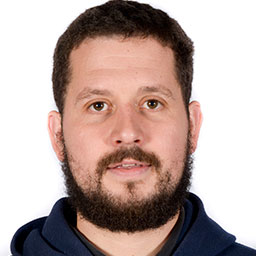
\includegraphics[width=4cm]{scarrign.png}
\end{figure}

\subsection*{Short Biography}
I am a PhD student in Computer Applications in Science and Engineering at the Barcelona Supercomputing Center. I hold a M.S. in Cognitive Sciences and a M.A. in History and Philosophy of Science. My work focus on the use of computer modeling and evolutionary method to study Complex Systems ranging from Evolutionary Biology to Human and Cultural Dynamics. Among different projects, I studied the evolution of specialization in swarm of simulated robots, the evolution of altruism in population of simulated social agents and the epistemological aspects of the use of computer simulations and computer models to understand Evolutionary Biology and Social Sciences. My actual PhD thesis explores the interactions between cultural evolution processes (social learning, biased copy,...) and Economic Dynamics (pricing, trading strategies,...) in actual and past societies.


\subsection*{Selected Bibliography}

\subsubsection*{Peer-reviewed Journals:}

\begin{itemize}
    \item  \bibentry{zibetti2015acaciaesanagentbasedmodelingandsimulationtoolforinvestigatingsocialbehaviorsinresourcelimitedtwodimensionalenvironments}

    \item  \bibentry{montanier2016behavioralspecializationinembodiedevolutionaryroboticswhysodifficult}
\end{itemize}



\subsubsection*{Peer-reviewed Proceedings of Conferences:}

\begin{itemize}
    \item  \bibentry{medernach2015evolutionary}  
    \item  \bibentry{carrignon2015modelingthecoevolutionoftradeandcultureinpastsocieties}
    \item  \bibentry{medernach2016evolution}  
\end{itemize}


\pagebreak

\bibliographystyle{alpha}
\nobibliography{../biblio/bib/SimonCarrignon}


\end{document}

